\section{MTSP}

% \begin{frame}{Multi-task Speaker Pre-training (MTSP)}
%     \frametitle{Multi-task Speaker Pre-training (MTSP)}
%     The goal of Multi-task Speaker Pre-training (MTSP) is to improve pronunciation clarity and naturalness through multi-task learning, thereby enhancing the quality of dubbing pronunciation.
%     \begin{itemize}
%         \item \textbf{TTS Task:} Learn accurate pronunciation representations from a text-to-speech corpus.
%         \item \textbf{MLM Prediction Task:} Learn contextual relationships between phonemes to better handle unseen text.
%     \end{itemize}
%     \textbf{Illustration of MTSP}
%     \begin{figure}[htpb]
%         \centering
%         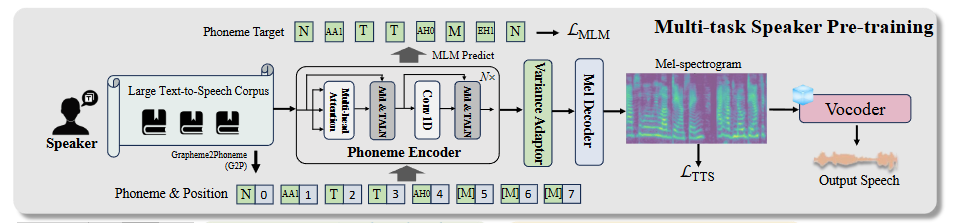
\includegraphics[width=0.8\textwidth]{figs/MSTP.png} % Replace with your image path
%         \caption{Illustration of Multi-task Speaker Pre-training}
%         \label{fig:mtsp}
%     \end{figure}
% \end{frame}
\begin{frame}{Multi-task Speaker Pre-training (MTSP)}
    \frametitle{Multi-task Speaker Pre-training (MTSP)}
    \textbf{Goal:} Improve pronunciation clarity and naturalness via multi-task learning.
    \begin{itemize}
        \item \textbf{TTS Task:} Learn accurate pronunciation from text-to-speech corpus.
        \item \textbf{MLM Task:} Capture phoneme context to handle unseen text.
    \end{itemize}
    \begin{figure}
        \centering
        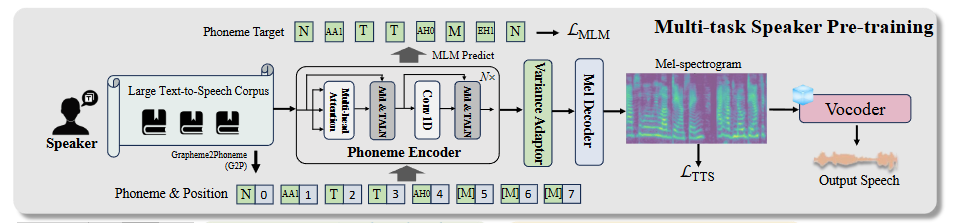
\includegraphics[width=0.8\textwidth]{figs/MSTP.png}
        \caption{Illustration of MTSP}
        \label{fig:mtsp}
    \end{figure}
\end{frame}

% \begin{frame}{TTS Task in MTSP}
%     \frametitle{TTS Task in MTSP}
%     \textbf{The TTS task enables the model to learn accurate pronunciation representations from a text-to-speech corpus} \\
%     Using an architecture similar to FastSpeech2, which includes a phoneme encoder, variance adaptor, and mel-decoder.
%     \begin{columns}[T] % Use top-aligned two columns
%         \column{0.6\textwidth} % Left column width is half of the text width
%         \begin{itemize}
%             \item Convert text to phoneme sequence: $T_p = \text{G2P}(T_o) $
%             \item The phoneme encoder extracts phoneme embeddings: $T_e = \text{PhonemeEncoder}(T_p) $
%             \item The variance adaptor models the prosody attributes of speech: $T_{\text{mel}} = \text{VarianceAdaptor}(E_{\text{ph}}, D_{\text{ph}}, P_{\text{ph}}, E_{\text{ph}})$
%         \end{itemize}
        
%         \column{0.4\textwidth} % Right column width is half of the text width
%         \begin{figure}[htpb]
%             \centering
%             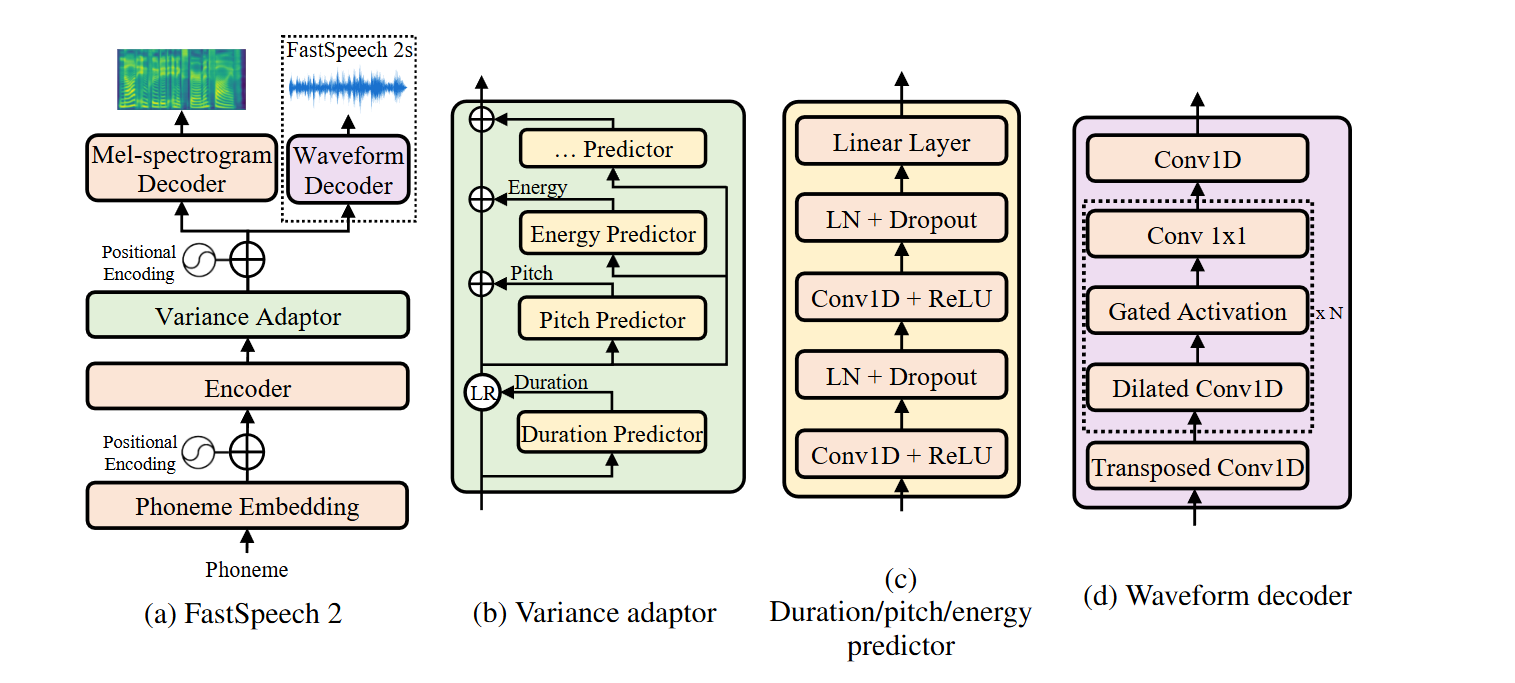
\includegraphics[width=\textwidth]{figs/fastSpeech架构图.png} % Replace with your image path
%             \caption{FastSpeech2 Architecture}
%             \label{fig:fastspeech2}
%         \end{figure}
%     \end{columns}
%     \vspace{1cm}
%     \textbf{Then predict the mel-spectrogram of the target speech and calculate the loss for the TTS task.}
% \end{frame}
\begin{frame}{TTS Task in MTSP}
    \frametitle{TTS Task in MTSP}
    \textbf{Objective:} Learn accurate pronunciation from text-to-speech corpus using FastSpeech2-like architecture.
    \begin{columns}[T] % Use top-aligned two columns
        \column{0.6\textwidth} % Left column width is 60% of the text width
        \begin{itemize}
            \item Convert text to phoneme sequence: $T_p = \text{G2P}(T_o)$
            \item Extract phoneme embeddings: $T_e = \text{PhonemeEncoder}(T_p)$
            \item Model prosody attributes: $T_{\text{mel}} = \text{VarianceAdaptor}(E_{\text{ph}}, D_{\text{ph}}, P_{\text{ph}}, E_{\text{ph}})$
        \end{itemize}
        
        \column{0.4\textwidth} % Right column width is 40% of the text width
        \begin{figure}[htpb]
            \centering
            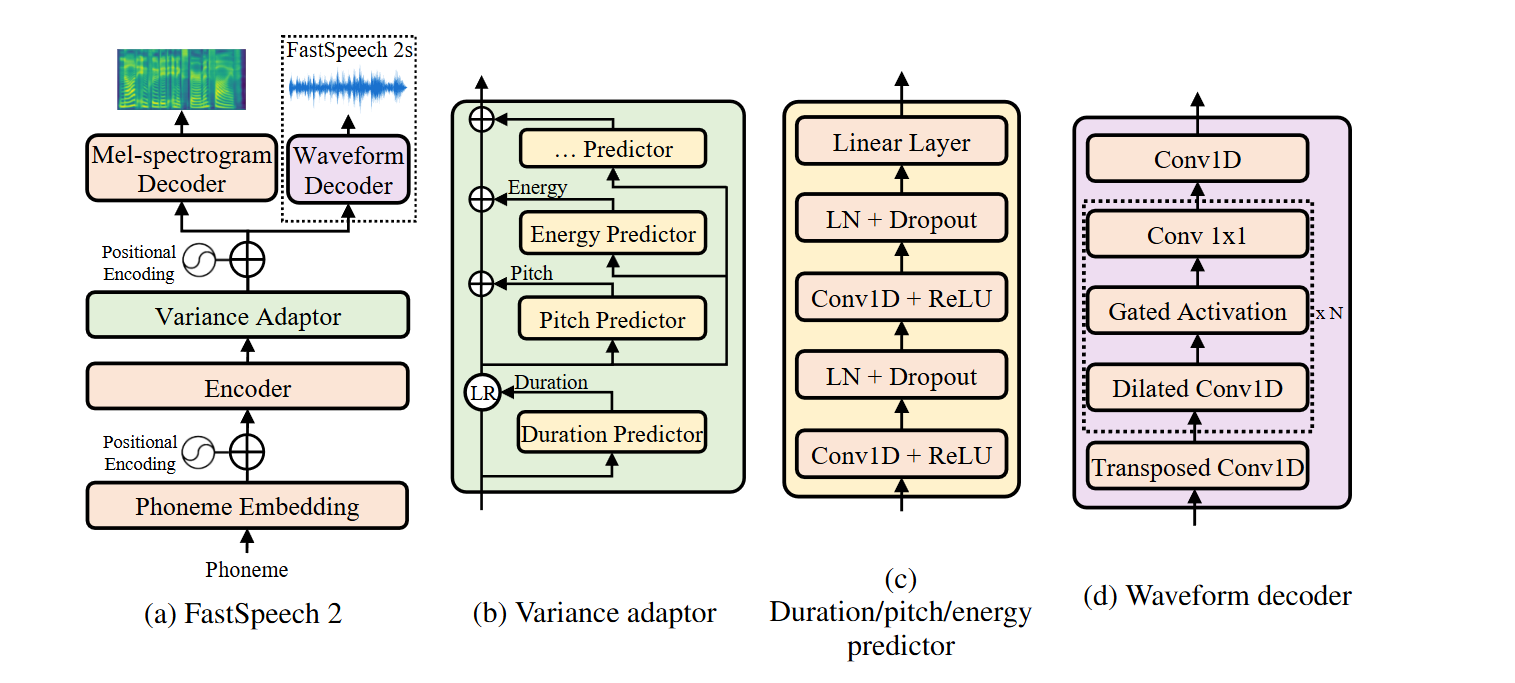
\includegraphics[width=\textwidth]{figs/fastSpeech架构图.png} % Replace with your image path
            \caption{FastSpeech2 Architecture}
            \label{fig:fastspeech2}
        \end{figure}
    \end{columns}
    \vspace{0.3cm}
    \textbf{Then predict the mel-spectrogram of the target speech and calculate the loss for the TTS task.}
\end{frame}

\begin{frame}{MLM Prediction Task in MTSP}
    \frametitle{MLM Prediction Task in MTSP}
    \textbf{The MLM prediction task helps the model learn contextual relationships between phonemes.}
    \begin{itemize}
        \item \textbf{Input:} Randomly masked phoneme sequence.
        \item \textbf{Processing:} Input to the phoneme encoder to predict the masked phonemes.
        \item \textbf{Output:} Predict the masked phonemes using linear projection and softmax function.
    \end{itemize}
    \textbf{MLM Prediction Task:}
    \begin{itemize}
        \item Predict the masked phonemes:
        \begin{equation}
            L_{\text{MLM}} = \text{CE}(\text{PhonemeEncoder}(T_{\text{masked}}), T_{\text{target}})
        \end{equation}
    \end{itemize}
\end{frame}


% \begin{frame}{Summary of MTSP}
%     \frametitle{Summary of MTSP}
%     \begin{itemize}
%         \item Multi-task Speaker Pre-training (MTSP) combines the Text-to-Speech (TTS) and Masked Language Model (MLM) tasks to improve the model's pronunciation quality and expressiveness.
%         \item The total loss function of MTSP integrates the losses of these two tasks, as shown in the formula:
%     \end{itemize}
%     \begin{equation}
%         \mathcal{L}_{MTSP} = \alpha_1 \cdot \mathcal{L}_{TTS} + \alpha_2 \cdot \mathcal{L}_{MLM},
%     \end{equation}
%     where, $\alpha_1$ and $\alpha_2$ are predefined hyperparameters, used to adjust the weights of the TTS and MLM tasks in the total loss.
% \end{frame}

\begin{frame}{Summary of MTSP}
    \frametitle{Summary of MTSP}
    \begin{itemize}
        \item \textbf{MTSP} combines \textbf{TTS} and \textbf{MLM} tasks to enhance pronunciation quality and expressiveness.
        \item Total loss function integrates losses of both tasks:
    \end{itemize}
    \begin{equation}
        \mathcal{L}_{MTSP} = \alpha_1 \cdot \mathcal{L}_{TTS} + \alpha_2 \cdot \mathcal{L}_{MLM},
    \end{equation}
    where $\alpha_1$ and $\alpha_2$ are hyperparameters adjusting task weights.
\end{frame}